\section{}
\[
H(s)=\frac{2\,s}{s^2+2s+1}=\frac{2\,s}{(s+1)^2}\,.
\]
\subsection{Bode-Diagramm}
\begin{center}
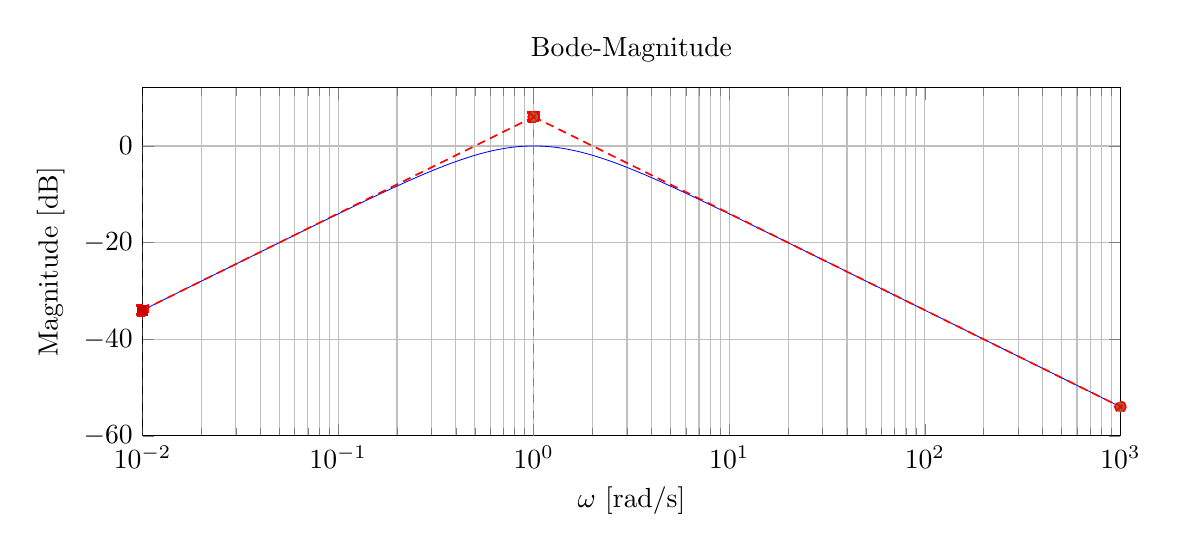
\begin{tikzpicture}
\begin{semilogxaxis}[
  width=14cm,height=6cm,
  xmin=1e-2,xmax=1e3,
  xlabel={$\omega$ [rad/s]},
  ylabel={Magnitude [dB]},
  grid=both,
  title={Bode-Magnitude}
]
\addplot[
  domain=1e-2:1e3,
  samples=700,
  mark=none,
  line width=0.3pt,
  blue
] {20*ln(2)/ln(10) + 20*ln(x)/ln(10) - 40*ln(sqrt(1 + x^2))/ln(10)};
\addplot+[domain=1e-2:1,samples=2,dashed,dash pattern=on 3pt off 2pt,line width=0.6pt,red] {20*ln(2)/ln(10) + 20*ln(x)/ln(10)};
\addplot+[domain=1:1e3,samples=2,dashed,dash pattern=on 3pt off 2pt,line width=0.6pt,red] {20*ln(2)/ln(10) - 20*ln(x)/ln(10)};
\draw[gray,dashed] (rel axis cs:0,0) -- (rel axis cs:0,1);
\draw[gray,dashed] (axis cs:1,\pgfkeysvalueof{/pgfplots/ymin}) -- (axis cs:1,\pgfkeysvalueof{/pgfplots/ymax});
\node[gray,anchor=south east] at (axis cs:1,\pgfkeysvalueof{/pgfplots/ymax}) {\scriptsize Pol $\omega_p=1$ (doppelt)};
\node[gray,anchor=south east] at (axis cs:1e-2,\pgfkeysvalueof{/pgfplots/ymax}) {\scriptsize Nullstelle im Ursprung};
\end{semilogxaxis}
\end{tikzpicture}
\vspace{6mm}
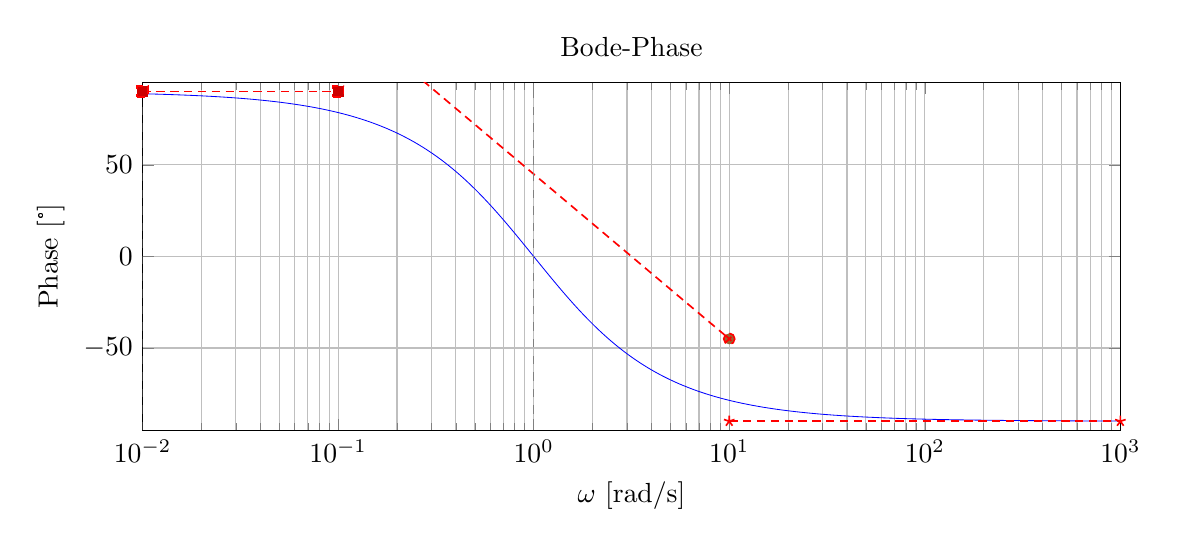
\begin{tikzpicture}
\begin{semilogxaxis}[
  width=14cm,height=6cm,
  xmin=1e-2,xmax=1e3,
  ymin=-95,ymax=95,
  xlabel={$\omega$ [rad/s]},
  ylabel={Phase [°]},
  grid=both,
  title={Bode-Phase}
]
\addplot[
  domain=1e-2:1e3,
  samples=700,
  mark=none,
  line width=0.3pt,
  blue
] {90 - 2*atan(x)};
\addplot+[domain=1e-2:1e-1,samples=2,dashed,dash pattern=on 3pt off 2pt,line width=0.6pt,red] {90};
\addplot+[domain=1e-1:1e1,samples=2,dashed,dash pattern=on 3pt off 2pt,line width=0.6pt,red] {45 - 90*ln(x)/ln(10)};
\addplot+[domain=1e1:1e3,samples=2,dashed,dash pattern=on 3pt off 2pt,line width=0.6pt,red] {-90};
\draw[gray,dashed] (rel axis cs:0,0) -- (rel axis cs:0,1);
\draw[gray,dashed] (axis cs:1,\pgfkeysvalueof{/pgfplots/ymin}) -- (axis cs:1,\pgfkeysvalueof{/pgfplots/ymax});
\node[gray,anchor=south east] at (axis cs:1,\pgfkeysvalueof{/pgfplots/ymax}) {\scriptsize Pol $\omega_p=1$ (doppelt)};
\node[gray,anchor=south east] at (axis cs:1e-2,\pgfkeysvalueof{/pgfplots/ymax}) {\scriptsize Nullstelle im Ursprung};
\end{semilogxaxis}
\end{tikzpicture}
\end{center}
\newpage
\subsection{Erklärung}
\vspace{5mm}
\begin{description}[leftmargin=1.2em,labelsep=.6em,font=\bfseries]
\item[Schritt 1] Nullstelle im Ursprung und Faktor $2$: für $\omega\ll1$ gilt $|H(\j\omega)|\approx 2\,\omega$ $\Rightarrow$ Startsteigung $+20\,\mathrm{dB/dec}$, Startniveau $20\log_{10}2\approx6.02\,\mathrm{dB}$; Startphase $\approx+90^\circ$.
\item[Schritt 2] Doppelter Pol bei $\omega=1\,\mathrm{rad/s}$: ab $\omega=1$ zusätzliche Steigungsänderung um $-40\,\mathrm{dB/dec}$; Netto-Slope für $\omega\gg1$ ist $-20\,\mathrm{dB/dec}$ ($|H|\sim 2/\omega$). Exakt am Eckpunkt: $|H(\j1)|=1\Rightarrow 0\,\mathrm{dB}$, also $20\log_{10}2-20\log_{10}2=0$ relativ zur Geraden. Phasenabfall der beiden Pole zusammen $180^\circ$ über $\omega\in[0.1,10]$; Näherung: $45^\circ-90^\circ\log_{10}\omega$.
\item[Schritt 3] Grenzverhalten: $\omega\ll1\Rightarrow |H|_{\mathrm{dB}}\approx 20\log_{10}2+20\log_{10}\omega$, $\angle H\approx+90^\circ$; $\omega\gg1\Rightarrow |H|_{\mathrm{dB}}\approx 20\log_{10}2-20\log_{10}\omega$, $\angle H\to-90^\circ$.
\end{description}

\vspace{0.5cm}
\medskip
\noindent\textbf{Stückweise Näherung}
\[
|H(\j\omega)|_{\mathrm{dB}}\approx
\begin{cases}
20\log_{10}2+20\log_{10}\omega,& \omega\ll1,\\[4pt]
\left.\;20\log_{10}2\;\right.-20\log_{10}2=0,& \omega=1,\\[4pt]
20\log_{10}2-20\log_{10}\omega,& \omega\gg1,
\end{cases}
\qquad
\]
\newpage